\documentclass[journal]{vgtc}                % final (journal style)
%\documentclass[review,journal]{vgtc}         % review (journal style)
%\documentclass[widereview]{vgtc}             % wide-spaced review
%\documentclass[preprint,journal]{vgtc}       % preprint (journal style)

%% Uncomment one of the lines above depending on where your paper is
%% in the conference process. ``review'' and ``widereview'' are for review
%% submission, ``preprint'' is for pre-publication, and the final version
%% doesn't use a specific qualifier.

%% Please use one of the ``review'' options in combination with the
%% assigned online id (see below) ONLY if your paper uses a double blind
%% review process. Some conferences, like IEEE Vis and InfoVis, have NOT
%% in the past.

%% Please use the ``preprint''  option when producing a preprint version
%% for sharing your article on an open access repository

%% Please note that the use of figures other than the optional teaser is not permitted on the first page
%% of the journal version.  Figures should begin on the second page and be
%% in CMYK or Grey scale format, otherwise, colour shifting may occur
%% during the printing process.  Papers submitted with figures other than the optional teaser on the
%% first page will be refused. Also, the teaser figure should only have the
%% width of the abstract as the template enforces it.

%% These few lines make a distinction between latex and pdflatex calls and they
%% bring in essential packages for graphics and font handling.
%% Note that due to the \DeclareGraphicsExtensions{} call it is no longer necessary
%% to provide the the path and extension of a graphics file:
%% 
\includegraphics{diamondrule} is completely sufficient.
%%
\ifpdf%                                % if we use pdflatex
  \pdfoutput=1\relax                   % create PDFs from pdfLaTeX
  \pdfcompresslevel=9                  % PDF Compression
  \pdfoptionpdfminorversion=7          % create PDF 1.7
  \ExecuteOptions{pdftex}
  \usepackage{graphicx}                % allow us to embed graphics files
  \DeclareGraphicsExtensions{.pdf,.png,.jpg,.jpeg} % for pdflatex we expect .pdf, .png, or .jpg files
\else%                                 % else we use pure latex
  \ExecuteOptions{dvips}
  \usepackage{graphicx}                % allow us to embed graphics files
  \DeclareGraphicsExtensions{.eps}     % for pure latex we expect eps files
\fi%

%% it is recomended to use ``\autoref{sec:bla}'' instead of ``Fig.~\ref{sec:bla}''
\graphicspath{{figures/}{pictures/}{images/}{./}} % where to search for the images

\usepackage{microtype}                 % use micro-typography (slightly more compact, better to read)
\PassOptionsToPackage{warn}{textcomp}  % to address font issues with \textrightarrow
\usepackage{textcomp}                  % use better special symbols
\usepackage{mathptmx}                  % use matching math font
\usepackage{times}                     % we use Times as the main font
\renewcommand*\ttdefault{txtt}         % a nicer typewriter font
\usepackage{cite}                      % needed to automatically sort the references
%\usepackage{tabu}                      % only used for the table example
\usepackage{booktabs}                  % only used for the table example
%% We encourage the use of mathptmx for consistent usage of times font
%% throughout the proceedings. However, if you encounter conflicts
%% with other math-related packages, you may want to disable it.

%% In preprint mode you may define your own headline. If not, the default IEEE copyright message will appear in preprint mode.
%\preprinttext{To appear in IEEE Transactions on Visualization and Computer Graphics.}

%% In preprint mode, this adds a link to the version of the paper on IEEEXplore
%% Uncomment this line when you produce a preprint version of the article 
%% after the article receives a DOI for the paper from IEEE
%\ieeedoi{xx.xxxx/TVCG.201x.xxxxxxx}

%% If you are submitting a paper to a conference for review with a double
%% blind reviewing process, please replace the value ``0'' below with your
%% OnlineID. Otherwise, you may safely leave it at ``0''.
\onlineid{0}

%% declare the category of your paper, only shown in review mode
\vgtccategory{Research}
%% please declare the paper type of your paper to help reviewers, only shown in review mode
%% choices:
%% * algorithm/technique
%% * application/design study
%% * evaluation
%% * system
%% * theory/model
\vgtcpapertype{please specify}

%% Paper title.
\title{FactExplorer: Embedding-based visual analysis of data fact space}

%% This is how authors are specified in the journal style

%% indicate IEEE Member or Student Member in form indicated below
\author{Roy G. Biv, Ed Grimley, \textit{Member, IEEE}, and Martha Stewart}
\authorfooter{
%% insert punctuation at end of each item
\item
 Roy G. Biv is with Starbucks Research. E-mail: roy.g.biv@aol.com.
\item
 Ed Grimley is with Grimley Widgets, Inc.. E-mail: ed.grimley@aol.com.
\item
 Martha Stewart is with Martha Stewart Enterprises at Microsoft
 Research. E-mail: martha.stewart@marthastewart.com.
}

%other entries to be set up for journal
\shortauthortitle{Biv \MakeLowercase{\textit{et al.}}: Global Illumination for Fun and Profit}
%\shortauthortitle{Firstauthor \MakeLowercase{\textit{et al.}}: Paper Title}

%% Abstract section.
%因为能够有效地传达来自数据的见解而不需要用户过多的精力投入,自动化地从多维数据中挖掘有趣的数据模式已经成为一种盛行的可视分析方法。然而,现有的创作工具摒弃了大多数的见解,只展示最具影响力的一小部分。这样不仅可能会丢失一些重要的见解(i.e.对算法而言不重要,但对用户而言是重要的),还缺失了见解的上下文联系。在本文中,一种能够衡量数据事件相似性的多因素嵌入方法被设计来生成整个事件空间的概览,从而解决事件上下文缺失。此外,一种故事线生成算法被设计来联系零散的事件来促进对事件空间的理解。这些想法被实现在一个叫作FactExplorer的可视分析系统中。最后,我们通过两个FactExplorer的使用场景、一项对照实验和对12个领域专家的一系列访谈来评估所提出的技术。我们的评价表明,FactExplorer有利于用户轻松高效地生成对数据空间的理解。
\abstract{Automatically discovering interesting data patterns from multi-dimensional data has become a prevalent visual analysis approach because of it's effectiveness in conveying facts from data without requiring excessive user efforts. 
Existing authoring tools mostly filter out facts that perform poorly in evaluation, and only show the most distinctive ones. 
However, it can not conclusively determine the role of facts with poor rating by algorithm in aiding exploration, and their absence also leads to a lack of context for significant facts.
To address these challenge, a multi-factor embedding approach, which can measure the similarity of data facts, is designed in this work to provide an overview of the whole facts and the context for each fact.
A multi-storyline generation algorithm is also designed to organize fact sequences from multiple perspectives to support an exploratory narrative 
These ideas are implemented in a visual analysis system named, FactExplorer. Finally, we evaluate the proposed technique through two FactExplorer usage scenarios and a user study. 
Our evaluation shows that FactExplorer helps users easily and efficiently to analyze and explore the fact space.%
} % end of abstract

%% Keywords that describe your work. Will show as 'Index Terms' in journal
%% please capitalize first letter and insert punctuation after last keyword
\keywords{Automatic design, data embedding, data story, human-computer interaction}

%% ACM Computing Classification System (CCS). 
%% See <http://www.acm.org/class/1998/> for details.
%% The ``\CCScat'' command takes four arguments.

\CCScatlist{ % not used in journal version
 \CCScat{K.6.1}{Management of Computing and Information Systems}%
{Project and People Management}{Life Cycle};
 \CCScat{K.7.m}{The Computing Profession}{Miscellaneous}{Ethics}
}

%% A teaser figure can be included as follows
\teaser{
  \centering
  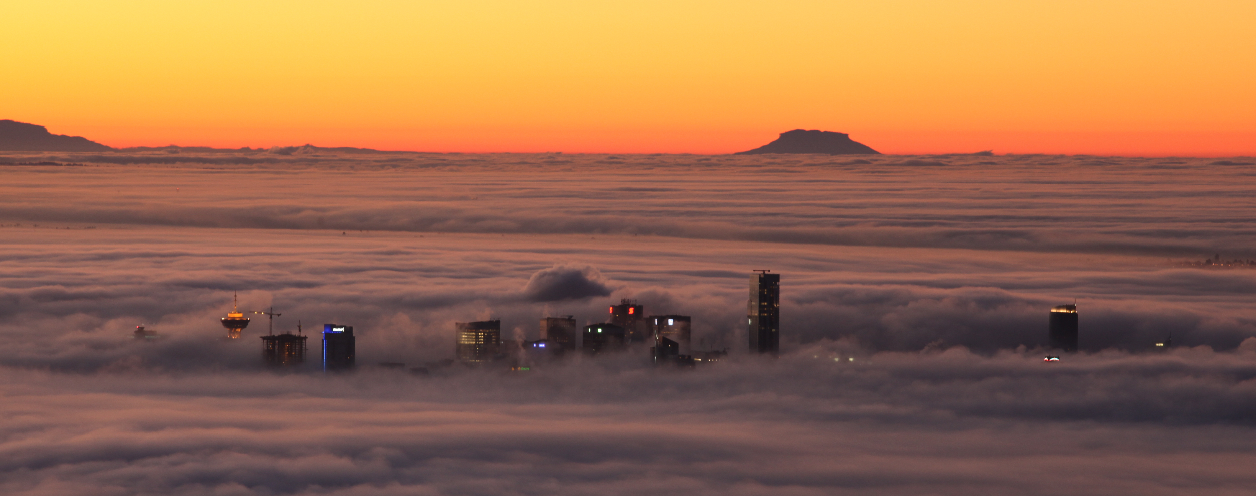
\includegraphics[width=\linewidth]{CypressView}
  \caption{In the Clouds: Vancouver from Cypress Mountain. Note that the teaser may not be wider than the abstract block.}
  \label{fig:teaser}
}

%% Uncomment below to disable the manuscript note
%\renewcommand{\manuscriptnotetxt}{}

%% Copyright space is enabled by default as required by guidelines.
%% It is disabled by the 'review' option or via the following command:
% \nocopyrightspace


\vgtcinsertpkg

%%%%%%%%%%%%%%%%%%%%%%%%%%%%%%%%%%%%%%%%%%%%%%%%%%%%%%%%%%%%%%%%
%%%%%%%%%%%%%%%%%%%%%% START OF THE PAPER %%%%%%%%%%%%%%%%%%%%%%
%%%%%%%%%%%%%%%%%%%%%%%%%%%%%%%%%%%%%%%%%%%%%%%%%%%%%%%%%%%%%%%%%

\begin{document}

\firstsection{Introduction} 
\maketitle
%目前,有一个多维数据分析领域中的新兴热门话题,自动化地传递见解,它能有效地降低了用户在探索数据中的努力,通过自动的见解发现,精心设计的布局和叙事结构,和引人入胜的可视映射。这些优点促进了自动传递见解创作工具的快速发展,例如datashot,data videos, 和calliope。上述的工作把用户从创作中解放出来,让他们更专注于高层的探索,这对于缺乏创作领域知识的普通受众是友好的,能够促进可视分析工具的普及。表格数据作为常见的信息存储介质,被选为本工作的关注点。在接下来的讨论中,我们用数据事件来表示表格数据中见解。
Currently, automatic insight delivery is emerging as a promising visual analysis approach in multi-dimensional data exploration. 
This technique can effectively reduce the effort of users in exploring data, through automatic insight discovery, well-designed layout and narrative structure, and engaging visual mapping. 
More and more researchers are attracted to create authoring tools for automated delivery of insights, such as datashot, data videos, and calliope. 
These tools liberate users from creation and allows them to focus on high-level exploration, that is friendly to ordinary audiences who are lack of domain-specific knowledge, and promotes the popularization of visual analysis tools.
Tabular data, as a common information storage medium, is selected as the focus of this work. In the following discussion, we utilize data fact to represent the insight in tabular data.

%根据一些评估指标来排序自动提取的见解并选择前top-k,是上述工作常采用的见解挖掘方法。然而,这样会导致大量的见解不可见。尽管这些事件在评估有不好的表现,但这不能定论他们在辅助用户理解中的作用。由于技术的限制,有一些见解难以被探查,如图中蓝色框外的圆点所示。和之前的工作相同,提升事件的检测能力目前不是我们的关注点。本工作更关注用户对事件空间的理解力以及他们能否有效顺利地定位到符合需求的事件。此外,上述方法的另一个局限是丢失了top-k见解的上下文信息,这不利于不同见解之间的过渡。总之,本工作面临的第一个挑战就是事件空间的概览以及支撑事件的上下文关系。
Ranking the data facts according to certain evaluation metrics and selecting the top-k ones is a common fact delivery approach utilized in aforementioned works. 
However, this will make a large number of facts invisible. Although these facts have a poor performance in the evaluation, it is not conclusive that their role in aiding users understanding.
Due to technical limitations, there are certain hard-to-find facts, as shown by the outermost dots in figure \ref{factspace}. 
As with the existing work, improving the fact detection ability is not our focus. This work focuses more on users' understanding of the fact space and whether they can effectively and smoothly locate the ones that meet their needs (dots in orange boxes in figure \ref{factspace}).
Furthermore, another limitation of the aforementioned approach is that the contextual information of the top-k facts is also lacking, which is not beneficial for users to switch between different facts.
In summary, the first challenge of this work is to support an overview of the whole fact space, as well as the context of each fact.

%数据故事将事件组装进精心设计的叙事结构已生成有意义的事件序列,是一种更加有效的传递见解的途径。已有工作针对研究如何构建优质的叙事序列,如xxxxxxxx。之前工作生成的故事线往往是在规则和评估表现最优的,但是这样的故事线视角单一和思考模式固定,留给用户的探索性不足。用户只能顺着算法最优的思考模式获取信息,而不是主动地按照自己的思考模式去探索。探索型的叙事不仅能够增强用户的趣味性还能揭露潜在的一些模式。本工作第二个挑战就是如何从多视角地生成故事线,增强用户探索的自主性,让用户能够决定叙事走向。
Data story, which assembles fact pieces into well-designed narrative structure to generate a meaningful sequence, is a more effective approach of delivering insights. 
Existing work has focused on researching how to construct high-quality narrative sequences. Such as,
Calliope incorporates a logic-oriented Monte Carlo tree search algorithm to progressively generate data facts and organize them in a logical sequence. 
Storylines, which generated in previous work, generally have good performance in evaluation or rule constraints. However, such storylines usually have a single narrative perspective and a fixed mindset, and can not provide a flexible exploration. 
Users can only receive information in the mindset that perform well in algorithm evaluation, instead of independently exploring according to their own mindset. 
Exploratory narratives can make user exploration more interesting and reveal more underlying patterns. 
Thence, the second challenge of this work is how to generate storylines from multiple perspectives, enhance the autonomy of exploration, and allow users to decide the direction of the narrative.
\begin{figure}[t]
	\centering
	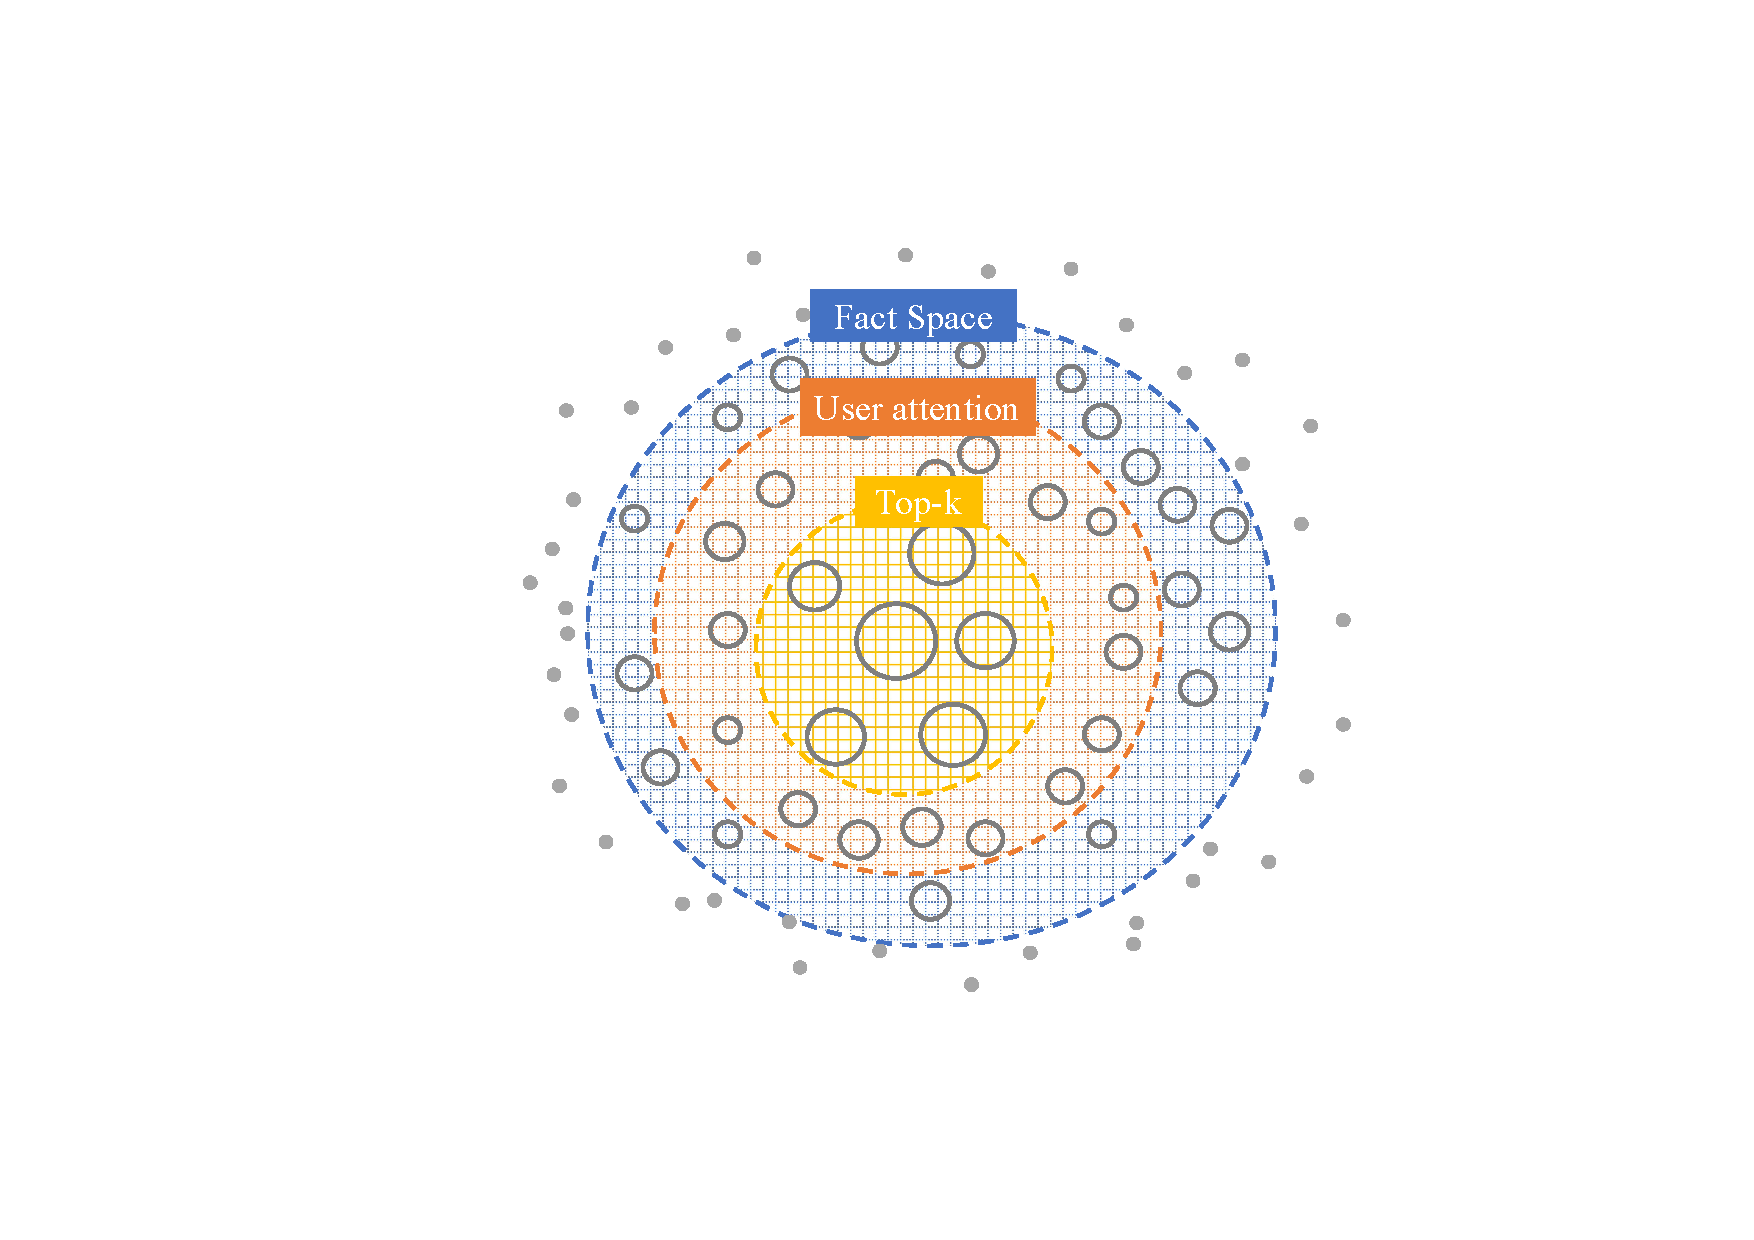
\includegraphics[width=0.5\textwidth]{figures/introduction.pdf}
	\caption{The illustration of fact space. The dots in blue box are the facts automatically extracted, orange box includes the facts that may be of interest to users, and top-k facts are in yellow box }
	\label{factspace}
\end{figure}

%为了解决上述挑战,我们提出了一个辅助探索事件空间的框架,框架由事件提取、事件嵌入和故事线提取三部分组成。我们引入了一种能够衡量数据事件相似性的双因素嵌入方法来将事件嵌入事件空间。一个新颖的变分编码器被采用来嵌入事件的视觉编码信息,根据之前的调查研究结果计算事件之间的逻辑距离来嵌入事件的逻辑信息。此外,我们还设计了一种新颖的多视角故事线生成算法。该算法分别从top-k个fact出发拓展故事线。一个事件路径搜索算法也被设计来寻找两个事件之间的过渡路径。最后,这些想法被实现在了一个用于探索事件空间的系统,FactExplorer。在系统中,我们还为用户设计了许多的交互通道,运行用户便捷地编辑事件和事件故事线。本文的主要贡献如下:
To address the above challenges, we propose a framework to assist in exploring the fact space, which consists of three parts: fact extraction, fact embedding, and storyline generation. 
In the fact embedding module, we introduce a two-factor embedding approach, which can measure the similarity of data facts, to embed facts into the fact space. 
More specifically, a novel variational encoder is employed to encode the visual style details of facts, and the logical relation of facts is embedded by computing the logical distance among facts based on the findings from previous work. 
Furthermore, we design a novel multi-storyline generation algorithm, which expands multi-perspective storylines from top-k facts respectively. A fact path search algorithm is also designed to seek a smooth and informative transition path from one fact to another.
Finally, these ideas are implemented in a fact space exploration system, FactExplorer. 
Certain interactions are also provided in the system to support flexible editing of facts and fact storylines.
The major contributions of this paper are as follows:
\begin{itemize}
%一个名为FactExplorer的可运行的系统,被设计来自动地挖掘表格数据背后的事件空间。合适的交互组件在系统中也被提供来支持灵活高效的探索
\item A runnable system named FactExplorer is designed to automatically build a fact space from tabular data. Appropriate interaction components are also provided in the system to support flexible and efficient exploration.
%一个用来将事件嵌入到事件空间的双因素(可视化样式和逻辑性)事件嵌入的方法。一个新颖的变分编码器模型被采用来嵌入可视化样式,逻辑性嵌入则通过计算事件之间的逻辑距离来实现,最后将它们聚合起来。
\item A two-factor (visual style and logical) fact embedding approach for embedding facts into the event space. A novel variational encoder model is utilized to embed visual styles, and logical embedding is achieved by computing the logical distance among facts, and finally aggregate these results to get fact embedding vector.
%一个多视角故事线生成算法来便捷用户的探索和增强用户对事件空间的记忆
\item An exploratory narrative approach is proposed to improve the flexibility and interest of exploration. More specifically, a multi-storyline generation algorithm is designed to generate multi-perspective storylines. A fact path search algorithm is also designed to seek a smooth and informative transition path from one fact to another.
\end{itemize}
\maketitle


\section{Relate Work} 
\subsection{Automatic Visualization} 
\subsection{Modeling Visualization Similarity} 
\subsection{Data-Driven Storytelling} 
\maketitle


\section{The Design Of FactExplorer} 
%在本章节中,我们讨论FactExplorer的设计目标以及System Pipeline,关于系统实现的详细内容将在下一章节阐述。
In this section, we discuss the design goals and system pipeline of FactExplorer. The details of the system implementation will be described in the next section.
\subsection{Design Goals} 
%FactExplorer的主要设计目标是最小化用户的努力去探索并且发现事件空间的有趣模式。更具体地,我们归纳出如下4个目标:
The main design goal of FactExplorer is to minimize users' efforts to explore and discover interesting patterns in the fact space. More specifically, we summarize the following four goals:

%1、确保提取数据事件的质量。系统应该确保提取的事件能覆盖大部分的原始数据空间、确保每个事件包括丰富的数据量、确保事件的可视化样式的多元性
\textbf{G1 Ensure the high quality of data facts.} The system should ensure that the extracted facts can cover most of the original data space, ensure that each fact includes a rich amount of data, and ensure that the visual styles of the facts are diverse.

%2、支持事件空间的语义概述。系统应该建模事件之间的相关性,并提供整个事件空间的概览。以促进用户对一个整体的理解。
\textbf{G2 Support a semantic overview of fact space.} The system should model relationships between facts and provide an overview of the entire fact space to facilitate users to develop a holistic understanding.

%3、将数据事件组织成故事线。系统应该将零散的事件组织成具有一定信息跨度、可视编码相关、逻辑相关的故事线。此外,系统还应该提供指定事件之间的过渡路径来进一步增强探索的灵活性
\textbf{G3 Organize data facts into storylines.} The system should organize fragmented facts into informative, encoding related, and logically related storylines. In addition, system should also provide a transition path between specified facts to incorporate real-time insights from users.

%4、支持便捷的用户交互。系统应该提供灵活的交互,以支持查询、筛选、查看特定的事件集合,并支持对生成数据事实和故事线进行全面编辑,以便用户从自己的视角去探索。
\textbf{G4 Support convenient user interactions.} The system should provide certain flexible interactive components to support querying, filtering, and viewing specific facts, and to enable comprehensive editing of generated facts and storylines for users.
\subsection{System Pipeline} 
%为了达到这些设计目标,我们采用面-线-点的层次结构来呈现数据事件。我们首先从表格数据中提取出事件(点)。然后将这些事件嵌入进事件空间,以使事件集的全局特征被揭露(面)。最后组装相关的事件成有意义的故事线(线)。图1显示了FactExplorer系统的pipline,它由三个核心模块组成
To achieve these design goals, we utilize a \textbf{plane-line-point} hierarchy to present data facts[cite]. We first extract the facts (\textbf{point}) from the tabular data. These facts are then embedded into the fact space to revealed the global features of fact collection (\textbf{plane}). Finally, related facts are assembled into meaningful storylines (\textbf{line}). Figure 1 shows the pipline of the FactExplorer system, which consists of three core modules

%事件提取。常用事件提取方法被采用来从表格数据中提取事件,处理过程包括:子空间切片、事件枚举、事件筛选、事件打分,这些过程都是系统自动完成的不需要用户干预。经过这个模块,底层的原始数据被转换成事件集合。
\textbf{Fact extraction.} Common fact extraction methods are utilized to extract facts from tabular data[cite]. The procedures executed include: subspace slicing, fact enumeration, fact screening, and fact scoring[\textbf{G1}]. These processes are automatically completed by the system , user only need to select the data attributes and fact types that participate in the fact extraction[\textbf{G4}]. After this module, the underlying raw data is converted into an fact collection.

%事件嵌入。在这个模块中,事件被嵌入到事件空间中,以提供一个事件集概览给用户。我们采用多通道嵌入的方法,和事件密切相关的属性(可视编码、逻辑性、偏差)都将被各自嵌入,最后这个单属性通道的嵌入通过不同权重聚合成最终的嵌入表达。
\textbf{Fact embedding.} In this module, facts are embedded into fact space to provide an overview of the fact collection. We adopt the method of multi-channel embedding, and factors closely related to the fact (visual encoding, logical, and deviation) will be embedded separately. Finally, these one-factor embeddings are aggregated into the final embedding by assigning different weights[\textbf{G2, G4}].

%故事线生成。在本模块,我们通过提取故事线来搭起事件间和事件簇间联系的桥梁,从而勾勒出事件空间中的结构。用户可以顺着故事线浏览事件空间中的干线,能够有效促进用户对事件空间的认知,加速探索进程。故事线提取的详细将在下个章节讨论。
\textbf{Storyline generation. }In this module, we delineate the structure in the fact space by extracting storylines to bridge the connections among facts and fact clusters[\textbf{G3}]. Users can browse the trunks along the storyline, it can effectively promote users' cognition of the fact space and accelerate the exploration process. The details of storyline extraction will be discussed in the next section.
\begin{figure}[h]
	\centering
	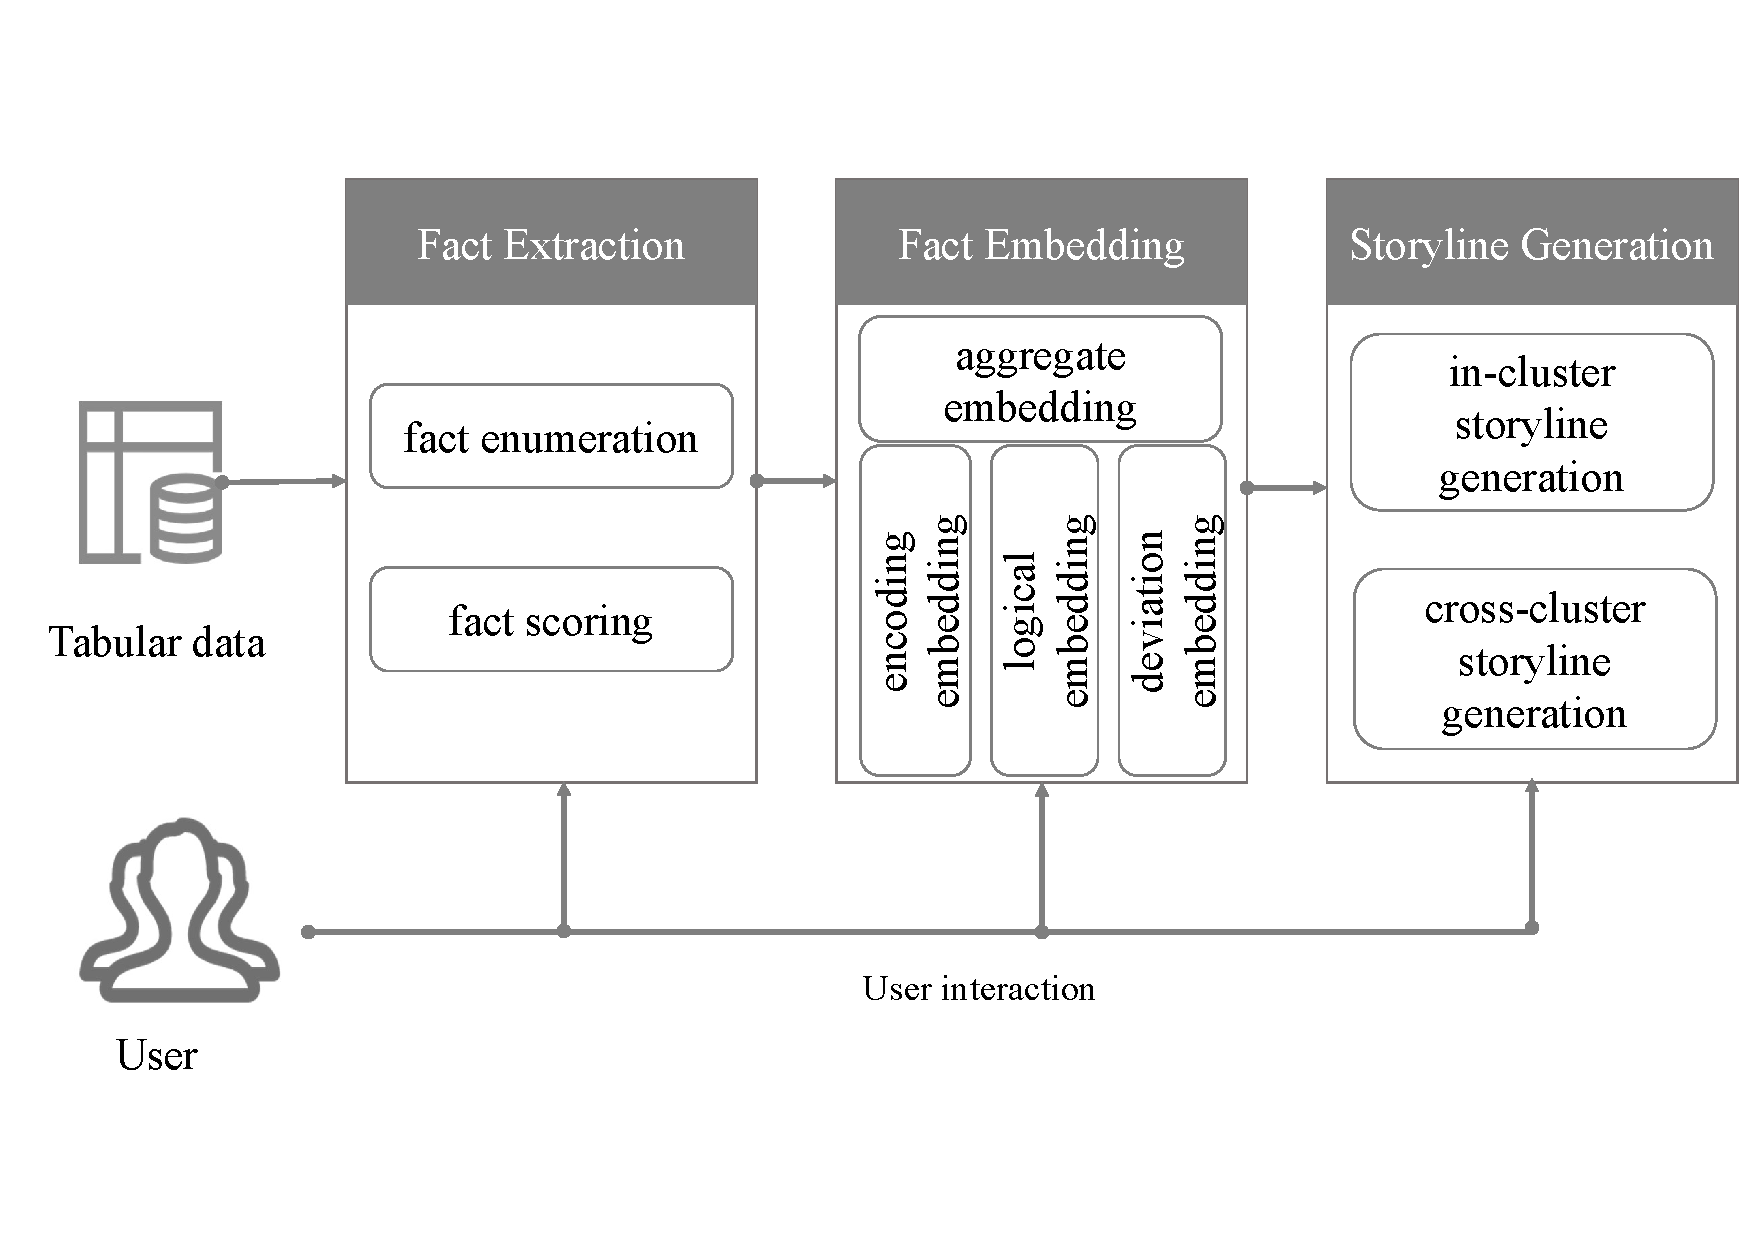
\includegraphics[width=0.5\textwidth]{figures/pipline.pdf}
	\caption{The processing pipeline of FactExplorer. First, FactExplorer automatically extracts facts from the tabular data and scores these facts. Next, these facts will be embedded into fact space from three perspectives: visual encoding, logical, and deviation. Finally, storylines will be extracted after clustering the facts.}
	\label{pipline}
\end{figure}
\maketitle


\section{FactExplorer System} 


\begin{figure}[ht]
	\centering
	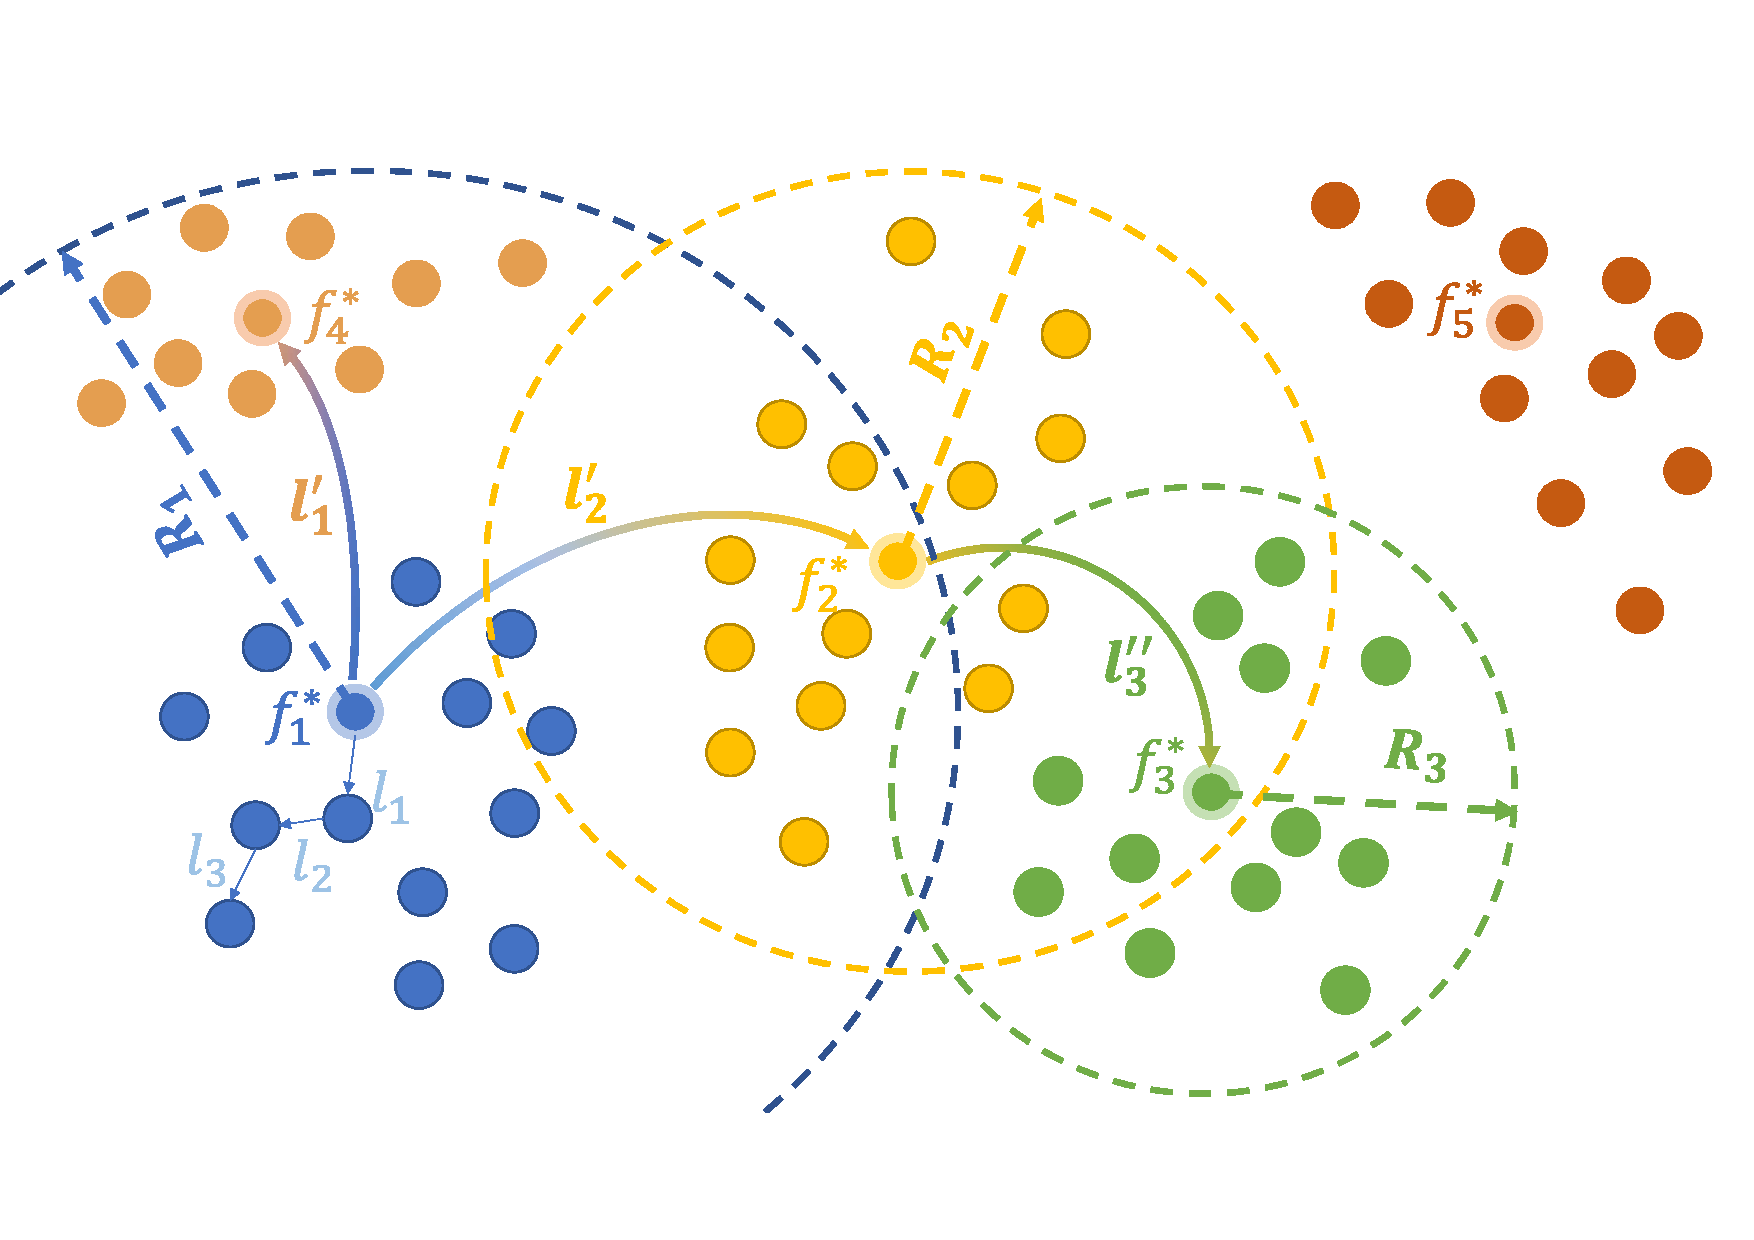
\includegraphics[width=0.5\textwidth]{figures/storyline.pdf}
	\caption{The processing pipeline of FactExplorer. First, FactExplorer automatically extracts facts from the tabular data and scores these facts. Next, these facts will be embedded into fact space from three perspectives: visual encoding, logical, and deviation. Finally, storylines will be extracted after clustering the facts.}
	\label{storyline}
\end{figure}
\maketitle


\section{Casestudy} 


\maketitle


\section{Userstudy} 


\maketitle


\section{Discussion} 


\maketitle


\section{Conslusion} 
%在本文中,我们介绍了FactExplorer, 一个用来辅助用户高效便捷地探索事件空间的系统。本系统,事件被自动从表格数据中提取。一个用来双因素(可视化样式和逻辑性)事件嵌入的方法被引入来将事件嵌入到事件空间,事件空间提供了所有事件地概览和每个事件的上下文。一个多故事线生成算法被设计来生成故事干线和支线。事件空间中的事件被合理地组织以便捷用户的探索和增强用户对事件空间的记忆。一些交互组件在系统中也被实现来支持用户灵活地编辑事件和事件故事线。通过两个个实例案例和一个用户研究,对该技术进行了评估。评价显示了FactExplorer的强大能力,并揭示了当前系统的几个局限性,这将在未来加以解决。
In this paper, we introduce FactExplorer, a system designed to help users efficiently and conveniently explore and analyze fact space. 
In this system, entire facts are automatically extracted from tabular data. 
A two-factor (visual style and logic) fact embedding approach is introduced to embed facts into the fact space, which provides an overview of all facts and the context of each fact. 
A multi-storyline generation algorithm is also designed to generate multiple perspectives storylines. The whole facts are organized well to promote exploration and deepen the impression of the fact space on the user. 
Certain interactive components are also implemented to support users to flexibly edit facts and storylines. 
These techniques proposed in this work is evaluated through two case studies and a user study. Finally, we discuss several limitations of the current system, which will be addressed in the future.

%\bibliographystyle{abbrv}
\bibliographystyle{abbrv-doi}
%\bibliographystyle{abbrv-doi-narrow}
%\bibliographystyle{abbrv-doi-hyperref}
%\bibliographystyle{abbrv-doi-hyperref-narrow}

\bibliography{template}
\end{document}

